\section{eBPF}

\begin{frame}{The ancestor: Berkeley Packet filter}
  \begin{itemize}
    \item BPF stands for Berkeley Packet Filter and was initially used
    for network packet filtering
    \item BPF is implemented and used in Linux to perform Linux Socket
    Filtering (see \kdochtml{networking/filter})
    \item tcpdump and Wireshark heavily rely on BPF (through libpcap) for
    packet capture
  \end{itemize}
\end{frame}

\begin{frame}{BPF in libpcap: setup}
  \begin{columns}
    \column{0.75\textwidth}
    \begin{itemize}
    \item tcpdump passes the capture filter string from the user to libpcap
    \item libpcap translates the capture filter into a binary program
      \begin{itemize}
      \item This program uses the instruction set of an abstract machine
        (the ``BPF instruction set'')
      \end{itemize}
    \item libpcap sends the binary program to the kernel via the
      \code{setsockopt()} syscall
    \end{itemize}
    \column{0.25\textwidth}
      \includegraphics[height=0.85\textheight]{slides/networking-ebpf/bpf-setup.pdf}
  \end{columns}
\end{frame}

\begin{frame}{BPF in libpcap: capture}
  \begin{columns}
    \column{0.55\textwidth}
    \begin{itemize}
    \item The kernel implements the BPF ``virtual machine''
    \item The BPF virtual machine executes the program for every packet
    \item The program inspects the packet data and returns a non-zero value
      if the packet must be captured
    \item If the return value is non-zero, the packet is captured in
      addition to regular packet processing
    \end{itemize}
    \column{0.45\textwidth}
      \includegraphics[height=0.80\textheight]{slides/networking-ebpf/bpf-capture.pdf}
  \end{columns}
\end{frame}

\begin{frame}
  \frametitle{eBPF (1/2)}
  \begin{itemize}
    \item \href{https://ebpf.io/}{eBPF} is a new framework allowing to run
    small user programs directly in the kernel, in a safe and efficient way. It
    has been added in kernel 3.18 but it is still evolving and receiving
    updates frequently.
    \item eBPF programs can capture and expose kernel data to userspace, and
    also alter kernel behavior based on some user-defined rules.
    \item eBPF is event-driven: an eBPF program is triggered and executed on a
    specific kernel event
    \item A major benefit from eBPF is the possibility to reprogram the kernel
    behavior, without performing kernel development:
    \begin{itemize}
      \item no risk of crashing the kernel because of bugs
      \item faster development cycles to get a new feature ready
    \end{itemize}
  \end{itemize}
  \center
\includegraphics[height=0.2\textheight]{slides/networking-ebpf/logo_ebpf.png}\\
  \tiny Image credits: \url{https://ebpf.io/}
\end{frame}

\begin{frame}
  \frametitle{eBPF (2/2)}
  \begin{itemize}
    \item The most notable eBPF features are:
    \begin{itemize}
      \item A new instruction set, interpreter and verifier
      \item A wide variety of "attach" locations, allowing to hook programs
      almost anywhere in the kernel
      \item dedicated data structures called "maps", to exchange data between
      multiple eBPF programs or between programs and userspace
      \item A dedicated \code{bpf()} syscall to manipulate eBPF programs and data
      \item plenty of (kernel) helper functions accessible from eBPF programs.
    \end{itemize}
  \end{itemize}
\end{frame}

\begin{frame}
  \frametitle{eBPF program lifecycle}
  \begin{center}
    \includegraphics[height=0.8\textheight]{slides/networking-ebpf/bpf_lifecycle.pdf}
  \end{center}
\end{frame}

\begin{frame}[fragile]
  \frametitle{Kernel configuration for eBPF}
  \begin{itemize}
    \item \kconfig{CONFIG_NET} to enable eBPF subsystem
    \item \kconfig{CONFIG_BPF_SYSCALL} to enable the \code{bpf()} syscall
    \item \kconfig{CONFIG_BPF_JIT} to enable JIT on programs and so increase performance
    \item \kconfig{CONFIG_BPF_JIT_ALWAYS_ON} to force JIT
    \item \kconfigval{CONFIG_BPF_UNPRIV_DEFAULT_OFF}{n} in \textbf{development} to
    allow eBPF usage without root
    \item You may then want to enable more general features to "unlock"
    specific hooking locations:
    \begin{itemize}
      \item \kconfig{CONFIG_KPROBES} to allow hooking programs on kprobes
      \item \kconfig{CONFIG_TRACING} to allow hooking programs on kernel tracepoints
      \item \kconfig{CONFIG_NET_CLS_BPF} to write packets classifiers
      \item \kconfig{CONFIG_CGROUP_BPF} to attach programs on cgroups hooks
    \end{itemize}
  \end{itemize}
\end{frame}

\begin{frame}[fragile]
  \frametitle{eBPF ISA}
  \begin{itemize}
    \item eBPF is a "virtual" ISA, defining its own set of instructions: load
    and store instruction, arithmetic instructions, jump instructions,etc
    \item It also defines a set of 10 64-bits wide registers as well as a
    calling convention:
    \begin{itemize}
      \item \code{R0}: return value from functions and BPF program
      \item \code{R1, R2, R3, R4, R5}: function arguments
      \item \code{R6, R7, R8, R9}: callee-saved registers
      \item \code{R10}: stack pointer
    \end{itemize}
  \end{itemize}
  \begin{block}{}
    \begin{minted}[fontsize=\scriptsize]{console}
; bpf_printk("Hello %s\n", "World");
      0:  r1 = 0x0 ll
      2:  r2 = 0xa
      3:  r3 = 0x0 ll
      5:  call 0x6
; return 0;
      6:  r0 = 0x0
      7:  exit
    \end{minted}
  \end{block}
\end{frame}

\begin{frame}[fragile]
  \frametitle{The eBPF verifier}
  \begin{itemize}
    \item When loaded into the kernel, a program must first be validated by the
    eBPF verifier.
    \item The verifier is a complex piece of software which checks eBPF
    programs against a set of rules to ensure that running those may not
    compromise the whole kernel. For example:
    \begin{itemize}
      \item a program must always return and so not contain paths which could
      make them "infinite" (e.g: no infinite loop)
      \item a program must make sure that a pointer is valid before
      dereferencing it
      \item a program can not access arbitrary memory addresses, it must use
      passed context and available helpers
    \end{itemize}
    \item If a program violates one of the verifier rules, it will be rejected.
    \item Despite the presence of the verifier, you still need to be careful when
    writing programs! eBPF programs run with preemption enabled (but CPU
    migration disabled), so they can still suffer from concurrency issues
    \begin{itemize}
      \item There are mechanisms and helpers to avoid those issues, like
        per-CPU maps types.
    \end{itemize}
  \end{itemize}
\end{frame}

\begin{frame}[fragile]
  \frametitle{Program types and attach points}
  \begin{itemize}
    \item There are different categories of hooks to which a program can be
    attached:
    \begin{itemize}
      \item an arbitrary kprobe
      \item a kernel-defined static tracepoint
      \item a specific perf event
      \item throughout the network stack
      \item and a lot more, see \ksym{bpf_attach_type}
    \end{itemize}
    \item A specific attach-point type can only be hooked with a set of
    specific program types, see \ksym{bpf_prog_type} and
    \kdochtml{bpf/libbpf/program_types}.
    \item The program type then defines the data passed to an eBPF program as
    input when it is invoked. For example:
    \begin{itemize}
      \item A \code{BPF_PROG_TYPE_TRACEPOINT} program will receive a structure
      containing all data returned to userspace by the targeted tracepoint.
      \item A \code{BPF_PROG_TYPE_SCHED_CLS} program (used to implement packets
      classifiers) will receive a \kstruct{__sk_buff}, the kernel
      representation of a socket buffer.
      \item You can learn about the context passed to any program type by
      checking \kfile{include/linux/bpf_types.h}
    \end{itemize}
  \end{itemize}
\end{frame}

\begin{frame}[fragile]
  \frametitle{eBPF maps}
  \begin{itemize}
    \item eBPF programs exchange data with userspace or other programs through
    maps of different nature:
    \begin{itemize}
      \item \code{BPF_MAP_TYPE_ARRAY}: generic array storage. Can be
      differentiated per CPU
      \item \code{BPF_MAP_TYPE_HASH}: a storage composed of key-value pairs.
      Keys can be of different types: \code{__u32}, a device type, an IP address...
      \item \code{BPF_MAP_TYPE_QUEUE}: a FIFO-type queue
      \item \code{BPF_MAP_TYPE_CGROUP_STORAGE}: a specific hash map keyed by a
      cgroup id. There are other types of maps specific to other object types
      (inodes, tasks, sockets, etc)
      \item etc...
    \end{itemize}
    \item For basic data, it is easier and more efficient to directly use eBPF
    global variables (no syscalls involved, contrary to maps)
  \end{itemize}
\end{frame}

\begin{frame}[fragile]
  \frametitle{The \code{bpf()} syscall}
  \begin{itemize}
    \item The kernel exposes a \code{bpf()} syscall to allow interacting with the
    eBPF subsystem
    \item The syscall takes a set of subcommands, and depending on the
    subcommand, some specific data:
    \begin{itemize}
      \item \ksym{BPF_PROG_LOAD} to load a bpf program
      \item \ksym{BPF_MAP_CREATE} to allocate maps to be used by a program
      \item \ksym{BPF_MAP_LOOKUP_ELEM} to search for an entry in a map
      \item \ksym{BPF_MAP_UPDATE_ELEM} to update an entry in a map
      \item etc
    \end{itemize}
    \item The syscall works with file descriptors pointing to eBPF resources.
    Those resources (program, maps, links, etc) remain valid while there is at least
    one program holding a valid file descriptor to it. Those are automatically cleaned
    once there are no user left.
    \item For more details, see  \manpage{bpf}{2}
  \end{itemize}
\end{frame}

\begin{frame}[fragile]
  \frametitle{Writing eBPF programs}
  \begin{itemize}
    \item eBPF programs can either be written directly in raw eBPF assembly or in
    higher level languages (e.g: C or rust), and are compiled using the clang
    compiler.
    \item The kernel provides some helpers that can be called from an eBPF program:
    \begin{itemize}
      \item \code{bpf_trace_printk} Emits a log to the trace buffer
      \item \code{bpf_map_{lookup,update,delete}_elem} Manipulates maps
      \item \code{bpf_probe_{read,write}[_user]} Safely read/write data from/to kernel or userspace
      \item \code{bpf_get_current_pid_tgid} Returns current Process ID and Thread group ID
      \item \code{bpf_get_current_uid_gid} Returns current User ID and Group ID
      \item \code{bpf_get_current_comm} Returns the name of the executable running in the
      current task
      \item \code{bpf_get_current_task} Returns the current \kstruct{task_struct}
      \item Many other helpers are available, see \manpage{bpf-helpers}{7}
    \end{itemize}
    \item Kernel also exposes kfuncs (see \kdochtml{bpf/kfuncs}), but contrary
    to bpf-helpers, those do not belong to the kernel stable interface.
  \end{itemize}
\end{frame}

\begin{frame}[fragile]
  \frametitle{Manipulating eBPF program}
  \begin{itemize}
    \item There are different ways to build, load and manipulate eBPF programs:
    \begin{itemize}
      \item One way is to write an eBPF program, build it with clang, and then load it,
      attach it and read data from it with bare \code{bpf()} calls in a custom
      userspace program
      \item One can also use \code{bpftool} on the built ebpf program to
      manipulate it (load, attach, read maps, etc), without writing any userspace tool
      \item Or we can write our own eBPF tool thanks to some intermediate libraries which handle most of the
      hard work, like libbpf
      \item We can also use specialized frameworks like BCC or bpftrace to really
      get all operations (bpf program build included) handled
    \end{itemize}
  \end{itemize}
\end{frame}

\begin{frame}[fragile]
  \frametitle{BCC}
  \begin{columns}
    \column{0.75\textwidth}
    \begin{itemize}
      \item BPF Compiler Collection (BCC) is (as its name suggests) a collection
            of BPF based tools.
      \item BCC provides a large number of ready-to-use tools written in BPF.
      \item Also provides an interface to write, load and hook BPF programs more
            easily than using "raw" BPF language.
      \item Available on a large number of architecture (Unfortunately, not ARM32).
      \begin{itemize}
        \item On debian, when installed, all tools are named \code{<tool>-bpfcc}.
      \end{itemize}
      \item BCC requires a kernel version >= 4.1.
      \item BCC evolves quickly, many distributions have old versions: you
            may need to compile from the latest sources
    \end{itemize}
  \column{0.25\textwidth}
  \vspace{0.5cm}
  
\includegraphics[height=0.2\textheight]{slides/networking-ebpf/logo_bcc.png}\\
  \tiny Image credits: \url{https://github.com/iovisor/bcc}
  \end{columns}
\end{frame}

\begin{frame}[fragile]
  \frametitle{BCC tools}
  \begin{center}
    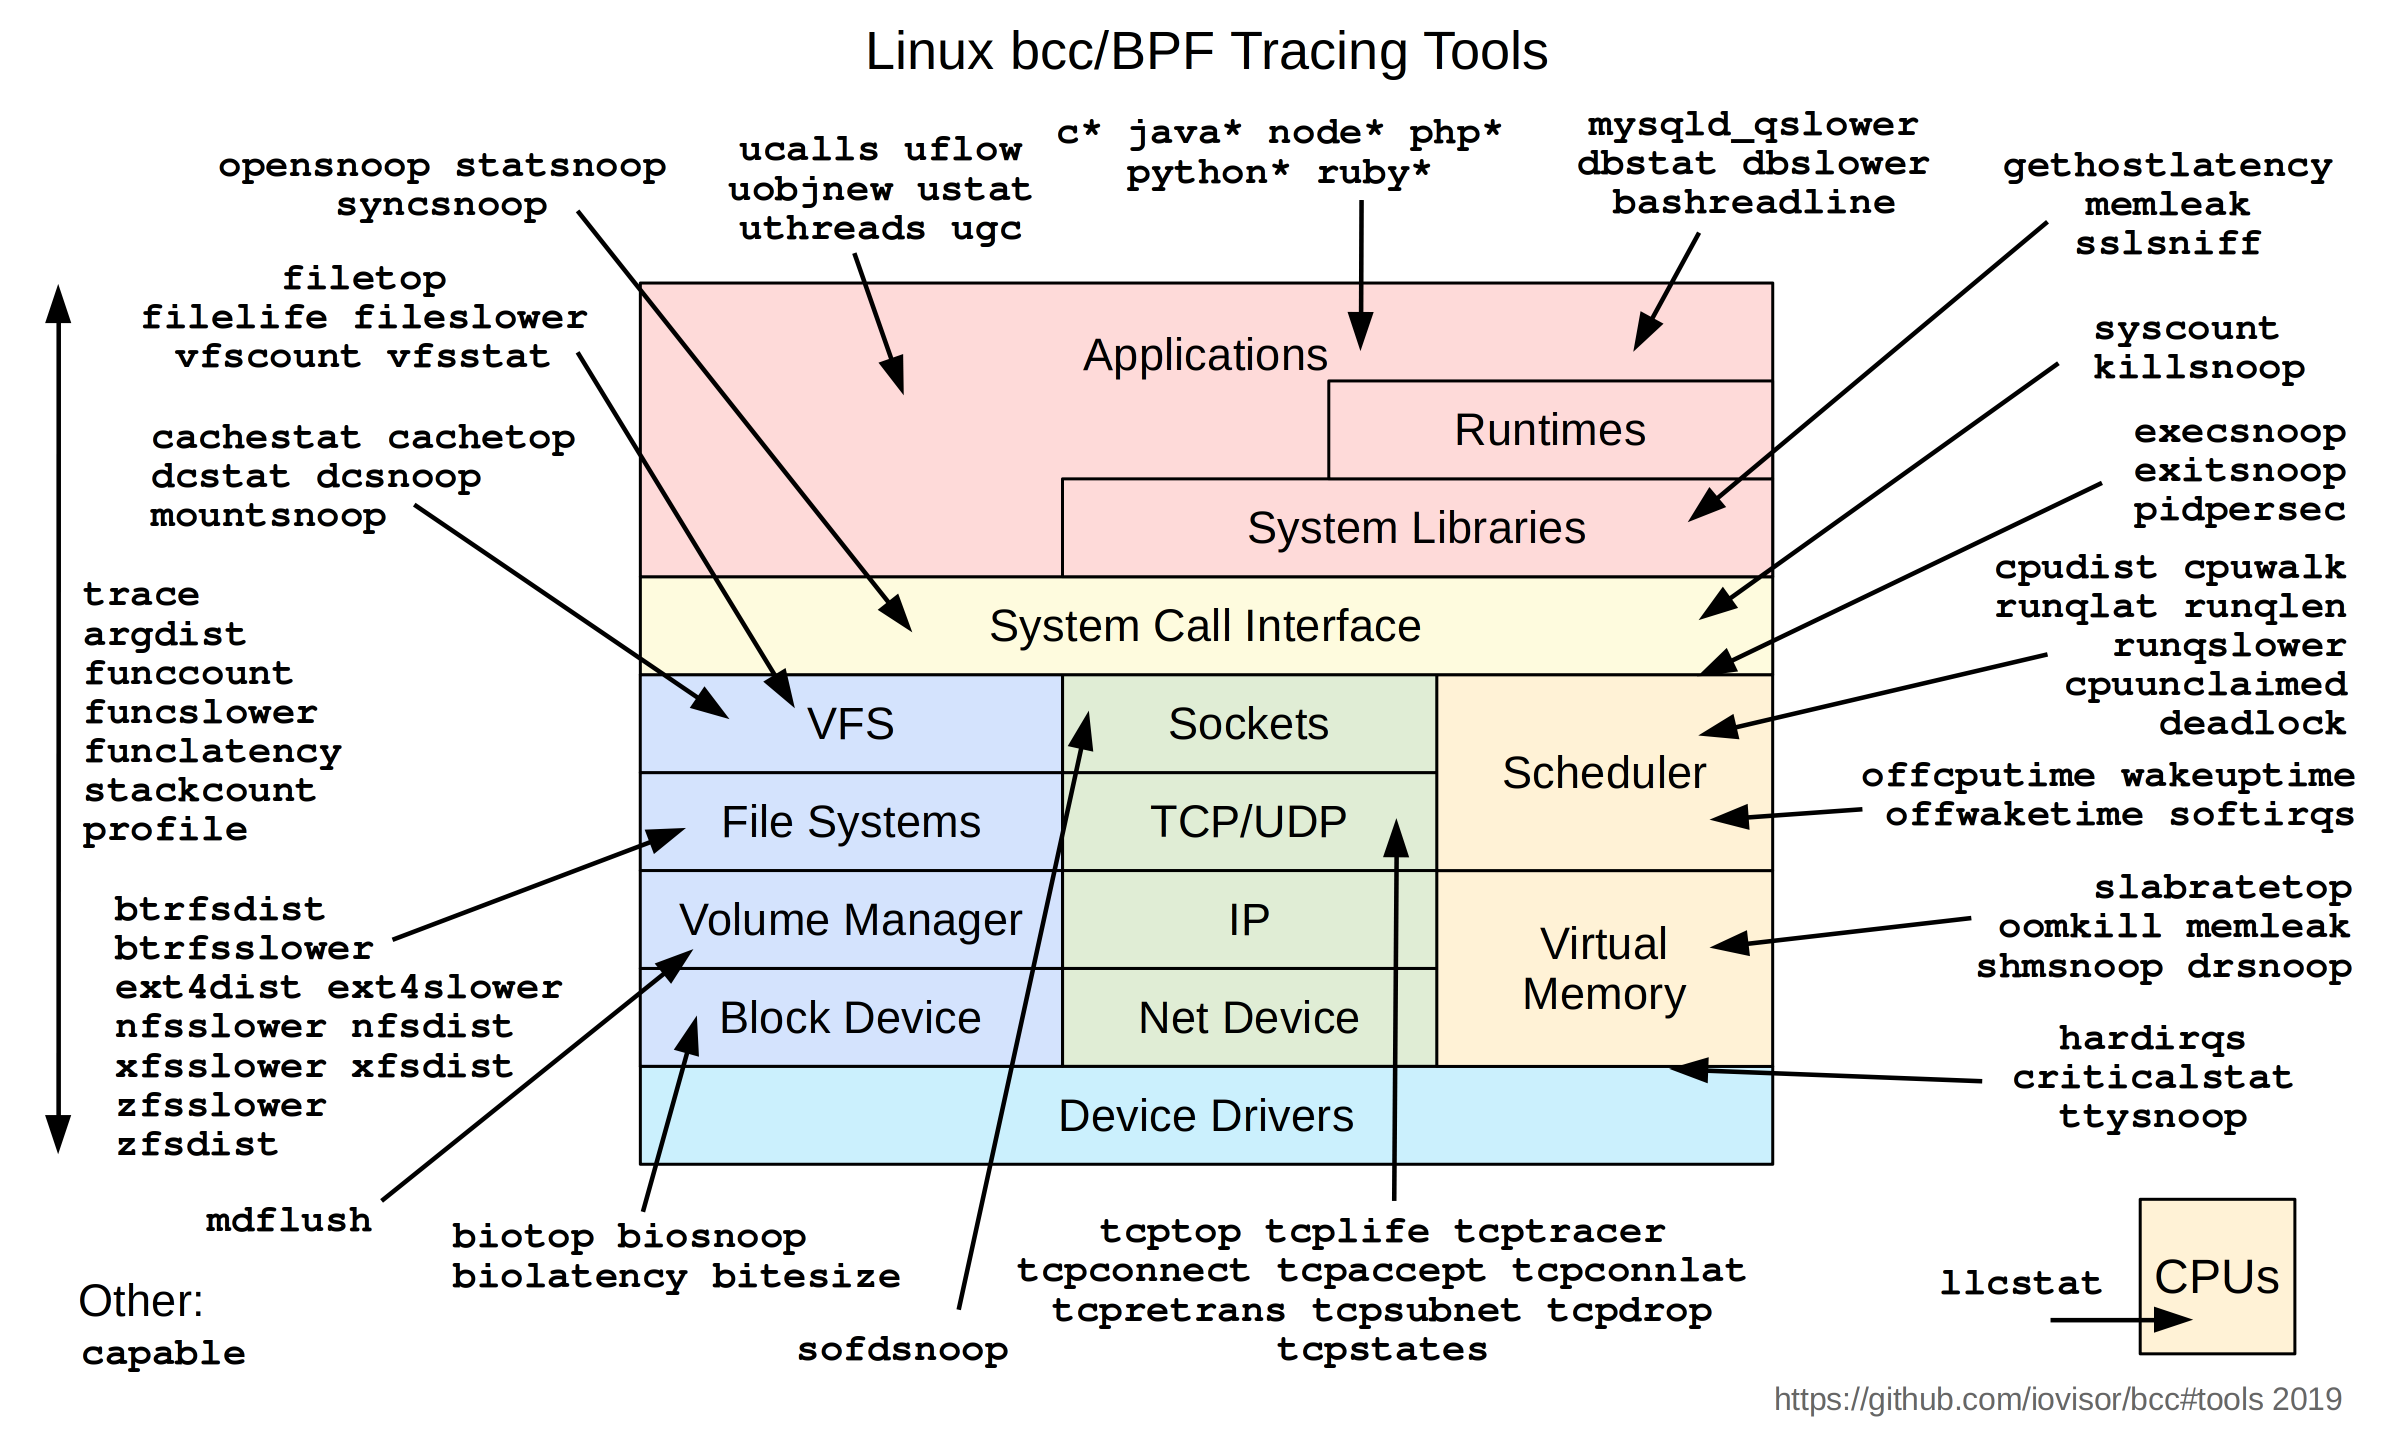
\includegraphics[height=0.8\textheight]{slides/networking-ebpf/bcc_tracing_tools_2019.png}\\
    \tiny Image credits: \url{https://www.brendangregg.com/ebpf.html}
  \end{center}
\end{frame}

\begin{frame}[fragile]
  \frametitle{BCC Tools example}
  \begin{itemize}
    \item \code{profile.py} is a CPU profiler allowing to capture stack traces of
          current execution. Its output can be used for flamegraph generation:
  \end{itemize}
  \begin{block}{}
    \begin{minted}[fontsize=\footnotesize]{console}
$ git clone https://github.com/brendangregg/FlameGraph.git
$ profile.py -df -F 99 10 | ./FlameGraph/flamegraph.pl > flamegraph.svg
    \end{minted}
  \end{block}
  \begin{itemize}
    \item \code{tcpconnect.py} script displays all new TCP connection live
  \end{itemize}
  \begin{block}{}
    \begin{minted}[fontsize=\footnotesize]{console}
$ tcpconnect
PID    COMM         IP SADDR            DADDR            DPORT
220321 ssh          6  ::1              ::1              22   
220321 ssh          4  127.0.0.1        127.0.0.1        22   
17676  Chrome_Child 6  2a01:cb15:81e4:8100:37cf:d45b:d87d:d97d 2606:50c0:8003::154 443  
[...]
    \end{minted}
  \end{block}
  \begin{itemize}
    \item And much more to discover at \url{https://github.com/iovisor/bcc}
  \end{itemize}
\end{frame}

\begin{frame}[fragile]
  \frametitle{Using BCC with python}
  \begin{itemize}
    \item BCC exposes a \code{bcc} module, and especially a \code{BPF} class
    \item eBPF programs are written in C and stored either in external files
    or directly in a python string.
    \item When an instance of the \code{BPF} class is created and fed with the
    program (either as string or file), it automatically builds, loads, and
    possibly attaches the program
    \item There are multiple ways to attach a program:
    \begin{itemize}
      \item By using a proper program name prefix, depending on the targeted
      attach point (and so the attach step is performed automatically)
      \item By explicitly calling the relevant attach method on the \code{BPF}
      instance created earlier
    \end{itemize}
  \end{itemize}
\end{frame}

\begin{frame}[fragile]
  \frametitle{Using BCC with python}
  \begin{itemize}
    \item Hook with a {\em kprobe} on the \code{clone()} system call and display \verb+"Hello, World!"+ each
          time it is called
  \end{itemize}
  \begin{block}{}
    \begin{minted}[fontsize=\small]{python}
#!/usr/bin/env python3

from bcc import BPF

# define BPF program
prog = """
int hello(void *ctx) {
    bpf_trace_printk("Hello, World!\\n");
    return 0;
}
"""
# load BPF program
b = BPF(text=prog)
b.attach_kprobe(event=b.get_syscall_fnname("clone"), fn_name="hello")
    \end{minted}
  \end{block}
\end{frame}

\begin{frame}[fragile]
  \frametitle{libbpf}
  \begin{itemize}
    \item Instead of using a high level framework like BCC, one can use libbpf to
    build custom tools with a finer control on every aspect of the program.
    \item libbpf is a C-based library that aims to ease eBPF programming thanks
    to the following features:
    \begin{itemize}
      \item userspace APIs to handle open/load/attach/teardown of bpf programs
      \item userspace APIs to interact with attached programs
      \item eBPF APIs to ease eBPF program writing
    \end{itemize}
    \item Packaged in many distributions and build systems (e.g.: Buildroot)
    \item Learn more at \url{https://libbpf.readthedocs.io/en/latest/}
  \end{itemize}
\end{frame}

\begin{frame}[fragile]
  \frametitle{eBPF programming with libbpf (1/2)}
  \begin{block}{\code{my_prog.bpf.c}}
    \begin{minted}[fontsize=\tiny]{C}
      #include <linux/bpf.h>
      #include <bpf/bpf_helpers.h>
      #include <bpf/bpf_tracing.h>

      #define TASK_COMM_LEN 16
      struct {
        __uint(type, BPF_MAP_TYPE_ARRAY);
        __type(key, __u32);
        __type(value, __u64);
        __uint(max_entries, 1);
      } counter_map SEC(".maps");

      struct sched_switch_args {
        unsigned long long pad;
        char prev_comm[TASK_COMM_LEN];
        int prev_pid;
        int prev_prio;
        long long prev_state;
        char next_comm[TASK_COMM_LEN];
        int next_pid;
        int next_prio;
      };
    \end{minted}
  \end{block}

  \begin{itemize}
  \item The fields to define in the \code{*_args} structure are obtained
    from the event description in \code{/sys/kernel/tracing/events} (see
    \href{https://elixir.bootlin.com/linux/v6.12/source/tools/testing/selftests/bpf/progs/test_stacktrace_map.c#L41}
         {this example})
  \end{itemize}
\end{frame}

\begin{frame}[fragile]
  \frametitle{eBPF programming with libbpf (2/2)}
  \begin{block}{\code{my_prog.bpf.c}}
    \begin{minted}[fontsize=\tiny]{C}
      SEC("tracepoint/sched/sched_switch")
      int sched_tracer(struct sched_switch_args *ctx)
      {
        __u32 key = 0;
        __u64 *counter;
        char *file;

        char fmt[] = "Old task was %s, new task is %s\n";
        bpf_trace_printk(fmt, sizeof(fmt), ctx->prev_comm, ctx->next_comm);

        counter = bpf_map_lookup_elem(&counter_map, &key);
        if(counter) {
                *counter += 1;
                bpf_map_update_elem(&counter_map, &key, counter, 0);
        }

        return 0;
      }

      char LICENSE[] SEC("license") = "Dual BSD/GPL";
    \end{minted}
  \end{block}
\end{frame}


\begin{frame}[fragile]
  \frametitle{Building eBPF programs}
  \begin{itemize}
    \item An eBPF program written in C can be built into a loadable object
    thanks to clang:
    \begin{block}{}
      \begin{minted}{console}
        $ clang -target bpf -O2 -g -c my_prog.bpf.c -o my_prog.bpf.o
      \end{minted}
    \end{block}
    \begin{itemize}
        \item The \code{-g} option allows to add debug information as well as
        BTF information
    \end{itemize}
    \item GCC can be used too with recent versions
    \begin{itemize}
      \item the toolchain can be installed with the \code{gcc-bpf} package in
      Debian/Ubuntu
      \item it exposes the \code{bpf-unknown-none} target
    \end{itemize}
    \item To easily manipulate this program with a userspace program based on libbpf,
    we need "skeleton" APIs, which can be generated with to \code{bpftool}
  \end{itemize}
\end{frame}

\begin{frame}[fragile]
  \frametitle{bpftool}
  \begin{itemize}
    \item \code{bpftool} is a command line tool allowing to interact with bpf
    object files and the kernel to manipulate bpf programs:
    \begin{itemize}
      \item Load programs into the kernel
      \item List loaded programs
      \item Dump program instructions, either as BPF code or JIT code
      \item List loaded maps
      \item Dump map content
      \item Attach programs to hooks (so they can run)
      \item etc
    \end{itemize}
    \item You may need to mount the bpf filesystem to be able to pin a program
    (needed to keep a program loaded after bpftool has finished running):
    \begin{block}{}
      \begin{minted}{console}
        $ mount -t bpf none /sys/fs/bpf
      \end{minted}
    \end{block}
  \end{itemize}
\end{frame}

\begin{frame}[fragile]
  \frametitle{bpftool}
  \begin{itemize}
    \item List loaded programs
  \end{itemize}
  \begin{block}{}
    \fontsize{10}{10}\selectfont
    \begin{minted}{console}
$ bpftool prog
348: tracepoint  name sched_tracer  tag 3051de4551f07909  gpl
loaded_at 2024-08-06T15:43:11+0200  uid 0
xlated 376B  jited 215B  memlock 4096B  map_ids 146,148
btf_id 545
    \end{minted}
  \end{block}
  \begin{itemize}
    \item Load and attach a program
  \end{itemize}
  \begin{block}{}
    \fontsize{10}{10}\selectfont
    \begin{minted}{console}
$ mkdir /sys/fs/bpf/myprog
$ bpftool prog loadall trace_execve.bpf.o /sys/fs/bpf/myprog autoattach
    \end{minted}
  \end{block}
  \begin{itemize}
    \item Unload a program
  \end{itemize}
  \begin{block}{}
    \fontsize{10}{10}\selectfont
    \begin{minted}{console}
$ rm -rf /sys/fs/bpf/myprog
    \end{minted}
  \end{block}
\end{frame}

\begin{frame}[fragile]
  \frametitle{bpftool}
  \begin{itemize}
    \item Dump a loaded program
  \end{itemize}
  \begin{block}{}
    \fontsize{8}{8}\selectfont
    \begin{minted}{console}
$ bpftool prog dump xlated id 348
int sched_tracer(struct sched_switch_args * ctx):
; int sched_tracer(struct sched_switch_args *ctx)
  0: (bf) r4 = r1
  1: (b7) r1 = 0
; __u32 key = 0;
  2: (63) *(u32 *)(r10 -4) = r1
; char fmt[] = "Old task was %s, new task is %s\n";
  3: (73) *(u8 *)(r10 -8) = r1
  4: (18) r1 = 0xa7325207369206b
  6: (7b) *(u64 *)(r10 -16) = r1
  7: (18) r1 = 0x7361742077656e20
[...]
    \end{minted}
  \end{block}
  \begin{itemize}
    \item Dump eBPF program logs
  \end{itemize}
  \begin{block}{}
    \fontsize{6}{6}\selectfont
    \begin{minted}{console}
$ bpftool prog tracelog
kworker/u80:0-11  [013] d..41  1796.003605: bpf_trace_printk: Old task was kworker/u80:0, new task is swapper/13
<idle>-0          [013] d..41  1796.003609: bpf_trace_printk: Old task was swapper/13, new task is kworker/u80:0
sudo-18640        [010] d..41  1796.003613: bpf_trace_printk: Old task was sudo, new task is swapper/10
<idle>-0          [010] d..41  1796.003617: bpf_trace_printk: Old task was swapper/10, new task is sudo
[...]
    \end{minted}
  \end{block}
\end{frame}

\begin{frame}[fragile]
  \frametitle{bpftool}
  \begin{itemize}
    \item List created maps
  \end{itemize}
  \begin{block}{}
    \fontsize{9}{9}\selectfont
    \begin{minted}{console}
$ bpftool map
80: array  name counter_map  flags 0x0
    key 4B  value 8B  max_entries 1  memlock 256B
    btf_id 421
82: array  name .rodata.str1.1  flags 0x80
    key 4B  value 33B  max_entries 1  memlock 288B
    frozen
96: array  name libbpf_global  flags 0x0
    key 4B  value 32B  max_entries 1  memlock 280B
[...]
    \end{minted}
  \end{block}
  \begin{itemize}
    \item Show a map content
  \end{itemize}
  \begin{block}{}
    \fontsize{9}{9}\selectfont
    \begin{minted}{console}
$ sudo bpftool map dump id 80
[{
  "key": 0,
  "value": 4877514
  }
]
    \end{minted}
  \end{block}
\end{frame}

\begin{frame}[fragile]
  \frametitle{bpftool}
  \begin{itemize}
    \item Generate libbpf APIs to manipulate a program
  \end{itemize}
  \begin{block}{}
    \fontsize{9}{9}\selectfont
    \begin{minted}{console}
$ bpftool gen skeleton trace_execve.bpf.o name trace_execve > trace_execve.skel.h
    \end{minted}
  \end{block}
  \begin{itemize}
    \item We can then write our userspace program and benefit from high level
    APIs to manipulate our eBPF program:
    \begin{itemize}
      \item instantiation of a global context object which will have references
      to all of our programs, maps, links, etc
      \item loading/attaching/unloading of our programs
      \item eBPF program directly embedded in the generated header as a byte
      array
    \end{itemize}
  \end{itemize}
\end{frame}

\begin{frame}[fragile]
  \frametitle{Userspace code with libbpf}
  \begin{block}{}
    \begin{minted}[fontsize=\tiny]{C}
      #include <stdlib.h>
      #include <stdio.h>
      #include <unistd.h>
      #include "trace_sched_switch.skel.h"

      int main(int argc, char *argv[])
      {
          struct trace_sched_switch *skel;
          int key = 0;
          long counter = 0;

          skel = trace_sched_switch__open_and_load();
          if(!skel)
              exit(EXIT_FAILURE);
          if (trace_sched_switch__attach(skel)) {
              trace_sched_switch__destroy(skel);
              exit(EXIT_FAILURE);
          }

          while(true) {
              bpf_map__lookup_elem(skel->maps.counter_map, &key, sizeof(key), &counter, sizeof(counter), 0);
              fprintf(stderr, "Scheduling switch count: %d\n", counter);
              sleep(1);
          }

          return 0;
      }
    \end{minted}
  \end{block}
\end{frame}

\begin{frame}
  \frametitle{eBPF programs portability (1/2)}
  \begin{itemize}
    \item Kernel internals, contrary to userspace APIs, do not expose stable APIs.
    This means that an eBPF program manipulating some kernel data may not work
    with another kernel version
    \item The CO-RE (Compile Once - Run Everywhere) approach aims to solve this issue
    and make programs portable between \textbf{kernel versions}. It relies on
    the following features:
    \begin{itemize}
      \item your kernel must be built with
      \kconfigval{CONFIG_DEBUG_INFO_BTF}{y} to have BTF data embedded. BTF is a
      format similar to dwarf which encodes data layout and functions
      signatures in an efficient way.
      \item your eBPF compiler must be able to emit BTF relocations (both clang
      and GCC are capable of this on recent versions, with the \code{-g} argument)
      \item you need a BPF loader capable of processing BPF programs based on BTF data and
      adjust accordingly data accesses: \code{libbpf} is the de-facto standard bpf
      loader
      \item you then need eBPF APIs to read/write to CO-RE relocatable
      variables. libbpf provides such helpers, like \code{bpf_core_read}
    \end{itemize}
    \item To learn more, take a look at
    \href{https://nakryiko.com/posts/bpf-core-reference-guide/}{Andrii
    Nakryiko's CO-RE guide}
  \end{itemize}
\end{frame}

\begin{frame}
  \frametitle{eBPF programs portability (2/2)}
  \begin{itemize}
    \item Despite CO-RE, you may still face different constraints on different
    kernel versions, because of major features introduction or change, since
    the eBPF subsystem keeps receiving frequent updates:
    \begin{itemize}
      \item eBPF tail calls (which allow a program to call a function) have
      been added in version 4.2, and allow to call another program only since
      version 5.10
      \item eBPF spin locks have been added in version 5.1 to prevent
      concurrent accesses to maps shared between CPUs.
      \item Different attach types keep being added, but possibly on different
      kernel versions when it depends on the architecture: fentry/fexit attach
      points have been added in kernel 5.5 for x86 but in 6.0 for arm32.
      \item Any kind of loop (even bounded) was forbidden until version 5.3
      \item \code{CAP_BPF} capability, allowing a process to perform eBPF tasks, has
      been added in version 5.8
    \end{itemize}
  \end{itemize}
\end{frame}

\begin{frame}[fragile]
\frametitle{eBPF for tracing/profiling}
  \begin{itemize}
    \item eBPF is a very powerful framework to spy on kernel internals: thanks
    to the wide variety of attach point, you can expose almost any kernel code path and data.
    \item In the mean time, eBPF programs remain isolated from kernel code,
    which makes it safe (compared to kernel development) and easy to use.
    \item Thanks to the in-kernel interpreter and optimizations like JIT compilation, eBPF is very well
    suited for tracing or profiling with low overhead, even in production
    environments, while being very flexible.
    \item This is why eBPF adoption level keeps growing for debugging, tracing
    and profiling in the Linux ecosystem. As a few examples, we find eBPF usage in:
    \begin{itemize}
      \item tracing frameworks like \href{https://github.com/iovisor/bcc}{BCC}
      and \href{https://github.com/bpftrace/bpftrace}{bpftrace}
      \item network infrastructure components, like
      \href{https://github.com/cilium/cilium}{Cilium} or \href{https://github.com/projectcalico/calico}{Calico}
      \item network packet tracers, like
      \href{https://github.com/cilium/pwru}{pwru} or
      \href{https://github.com/feiskyer/dropwatch}{dropwatch}
      \item And many more, check \href{https://ebpf.io/applications/}{ebpf.io}
      for more examples
    \end{itemize}
  \end{itemize}
\end{frame}

\begin{frame}[fragile]
  \frametitle{eBPF: resources}
  \begin{itemize}
     \item BCC tutorial:
     \url{https://github.com/iovisor/bcc/blob/master/docs/tutorial_bcc_python_developer.md}
     \item libbpf-bootstrap: \url{https://github.com/libbpf/libbpf-bootstrap}
    \item A Beginner’s Guide to eBPF Programming - Liz Rice, 2020
    \begin{itemize}
      \item Video: \url{https://www.youtube.com/watch?v=lrSExTfS-iQ}
      \item Resources: \url{https://github.com/lizrice/ebpf-beginners}
    \end{itemize}
  \end{itemize}
  \begin{center}
     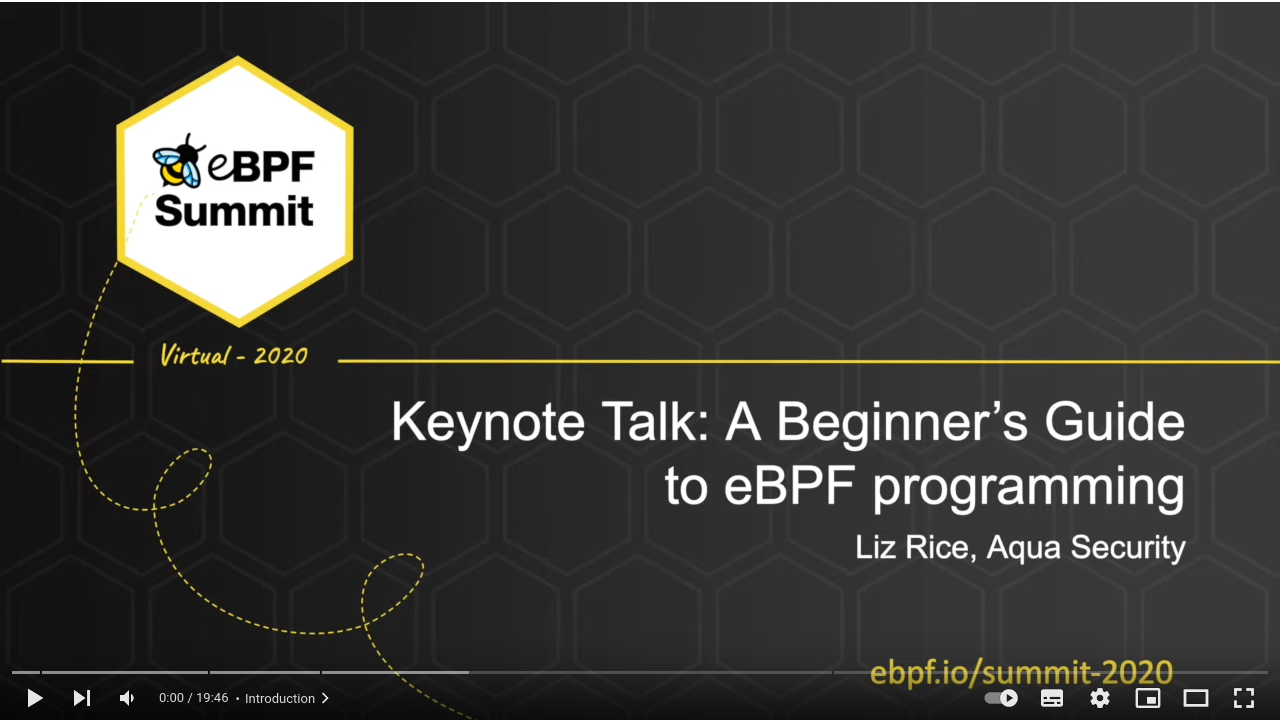
\includegraphics[height=0.4\textheight]{slides/networking-ebpf/ebpf_liz_rice_2020.png}
  \end{center}
\end{frame}



% eBPF principle
% Writing, compiling and loading eBPF progs
% Main hooks
